\chapter{Signal Extraction}
In this chapter, the procedure for signal yield extraction is presented. We use the framework of \texttt{RooFit} \cite{verkerke2006roofit} where we define 2D histogram templates in \vars, based on MC, for signal and several types of background. Using these templates, the independent full sample is fitted with the binned extended maximum likelihood (ML) fit, so that the individual template ratios and their sum describe the fitted sample as best as possible. In particle physics we are often dealing with low numbers of events and need to account for the Poisson nature of the data, therefore we use the likelihood fit, since it takes the Poisson errors into account, unlike the $\chi^2$ fit, where the errors are assumed to be Gaussian. In this procedure, we attempt to find the parameter values that maximize the likelihood function, given the observations.

If $P(n\vert\vec \alpha)$ is the probability of measuring $n$ candidates, where $\vec \alpha$ is a set of parameters on which $P$ depends, we can define the likelihood function $L$ for a series of such measurements (i.e., bins in histogram) $n_i$ based on Poisson statistics as
\begin{equation}
\label{eq:ML}
L(\vec \alpha) = \prod_{i=1} P(n_i|\vec \alpha) = \prod_{i=1} \frac{\mu_i^{n_i}\mathrm{e}^{-\mu_i}}{n_i!},
\end{equation}
where $\mu_i$ is the expected value for each measurement. It is also common to search for the minimum of the negative value of $\ln L$, or negative log-likelihood (NLL), as
\begin{equation}
\label{eq:NLL}
\mathcal{L}(\vec \alpha) = -\ln L(\vec \alpha) = -\sum_{i}\ln \left(\frac{\mu_i^{n_i}\mathrm{e}^{-\mu_i}}{n_i!}\right) = \sum_{i}\ln(n_i!) + \mu_i - n_i\ln(\mu_i).
\end{equation}
Maximizing $L$ or minimizing $\mathcal{L}$ gives us a maximum likelihood estimate of the set of parameters $\vec \alpha_{ML}$ which best describe the observed data. 

The ML method provides a method to estimate the fit uncertainty. This is especially useful if the log-likelihood has a non-parabolic shape, which leads to asymmetric errors. We calculate the errors using the \texttt{MINOS} algorithm from the \texttt{MINUIT} package \cite{James:1994vla}, which is implemented in RooFit. The algorithm follows the log-likelihood function out of the minimum to find the appropriate intervals of confidence for each parameter, taking the parameter correlations into account. 

To estimate the goodness of the likelihood fit, one option is to generate toy MC experiments and obtain the expected log-likelihood distribution. Likelihood fits, however, also offer another way to test the goodness of fit via the likelihood ratio (LR), where we compare the likelihood obtained under the ML parameters $\vec\alpha_{ML}$, to the likelihood obtained under the null hypothesis parameters $\vec\alpha_{H_0}$. This determines how likely the data is under one model than the other. We define the LR test as
\begin{equation}
\label{eq:lr}
\lambda = -2\ln\left(\frac{L(\vec \alpha_{ML})}{L(\vec \alpha_{H_0})}\right) = -2 \left[ \ln L(\vec \alpha_{ML}) - L(\vec \alpha_{H_0})\right] \sim \chi^2_q,
\end{equation}
which asymptotically behaves as the $\chi^2_q$ distribution with $q=m-n$ degrees of freedom, where $m$ and $n$ are degrees of freedom of $L(\vec \alpha_{ML})$ and $L(\vec \alpha_{H_0})$, respectively. In particle physics we usually study a specific decay and try to perform measurements of the signal yield, so the null hypothesis in this case is that we expect to observe no signal. This means that for the null hypothesis we fix the expected signal yield parameter to zero, while leaving the other parameters of $\vec\alpha_{H_0}$ the same as in $\vec\alpha_{ML}$, which results in $n = m-1$ degrees of freedom and in their difference $q = m -n = 1$. For such a simple $LR$ test of a single parameter the LR test then follows the $\chi^2$ distribution with $1$ degree of freedom. In this case we can define the fit significance from the $\chi^2$ value in units of $\sigma$ as
\begin{equation}
\mathrm{Significance} = \sqrt{\lambda} = \sqrt{\chi^2}.
\end{equation}

\section{Fit Setup}
We perform 10 fits to each stream of MC, where 9 streams were used for the creation of the templates and the remaining stream was used as fitted data. When fitting real data, all available MC was used for creating the templates. The full signal MC sample was used for the signal template definition in case of MC as well as data fits. The signal part of the \texttt{ulnu} sample was not used in template construction, it was only used as a part of the fitted sample. 

The same MC samples are used for template construction as described in chapter \ref{sec:data-and-monte-carlo-samples},
\begin{itemize}
	\item signal MC,
	\item 10 streams of \texttt{charged} and \texttt{mixed} $B \bar B$ background,
	\item 6 streams of $c \bar c$ (\texttt{charm}) and other $q \bar q$ (\texttt{uds}) background,
	\item \texttt{ulnu} sample, corresponding to $20\times$ integrated luminosity of the full Belle dataset,
	\item \texttt{rare} sample, corresponding to $50\times$ integrated luminosity of the full Belle dataset.
\end{itemize}

\subsection{Control Fit}\label{sec:control-fit}
$B \bar B$ background composition in control region is shown in Figure \ref{fig:cs_bkg_after}. Due to the strict cut of the $m_{KK}$ around the $D^0$ mass window, most of the decays with a $D^0$ proceed via $D^0 \to K^+K^-$ decay. In this case, the following fit templates are chosen
\begin{itemize}
	\item signal template,
	\item $q \bar q$ template,
	\item $C_0:~B^+ \to \bar{D} {}^0 \ell^+ \nu,~D^0 \to K^-K^+$ (control decay),
	\item $C_1:~B \to \bar{D} {}^* \ell^+ \nu,~D^0 \to K^-K^+$,
	\item other $B \bar B$ BKG template.
\end{itemize}
In control fits, all template shapes are fixed and the yields of all templates are floated, except for the signal template, which is expected to be very close to zero and is fixed to the expected MC yield. Additionally, since the $C_0$ and $C_1$ decays are well known and measured, we make use of this fact in the form of a ratio $N_{C_1}/N_{C_0}$, which is fixed to the MC value in case of the MC fit and constrained to the measured value in case of fits to real data. The ratio is implemented based on the decay channels shown in Table \ref{tab:cs_constraint_table} and is defined as
\begin{equation}
r_1 = \frac{\left(\sum_j N_{1j}\times \rho_{1j} \right)}{N_{00} \times \rho_{00}},
\label{eq:cs_fix}
\end{equation}
where $j$ runs over all channels in the category $C_1$ and where $\rho_{ij}$ is the branching ratio correction factor for the specific channel $N_{ij}$, which incorporates information from world measurements. It is defined as 
\begin{equation}
\rho = \frac{\mathcal{B}^{PDG}}{\mathcal{B}^{GEN}},
\label{eq:br_fix}
\end{equation}
where $\mathcal{B}^{PDG}$ is the measured branching ratio and $\mathcal{B}^{GEN}$ is the branching ratio value used in MC generation. The branching ratio correction factor has been implemented due to differences between measured and MC branching ratio values. Each branching ratio measurement serves as a constraint used in the fit. All branching ratio constraints in the control fit are shown in Table \ref{tab:cs_br_constraint_table}. The measured values are cited only for the $B^0$ decay mode, where isospin symmetry has been assumed. The corresponding $B^+$ branching ratios can be calculated as
\begin{equation}
\mathcal{B}(B^+) = \mathcal{B}(B^0) \times \tau_{B^+/B^0},
\end{equation}
where $\tau_{B^+/B^0}$ is the ratio of $B$-meson decay times, which is measured to be \cite{Amhis:2016xyh}
\begin{equation}
\tau_{B^+/B^0} = 1.076 \pm 0.004.
\end{equation}

\begin{table}[H]
	\centering
	\begin{tabular}{|l|l|l|l|l|}
		\hline
		Category & Channel & $B$ Decay Mode & $D$ Decay Mode & $N_{MC}$ \\
		\hline
		$C_0$ & $N_{00}$ & $B^+ \to \bar D {}^{0} \ell^+ \nu$ & $D^0 \to K^-K^+$ & $1182 \pm 34$\\
		\hline
		\hline
		\multirow{2}{*}{$C_1$} & $N_{10}$ & $B^+ \to \bar D {}^{*0} \ell^+ \nu$ & $D^0 \to K^-K^+$ & $1455\pm38$\\
		\cline{2-5}
		& $N_{11}$ & $B^0 \to D {}^{*-} \ell^+ \nu$ & $D^0 \to K^-K^+$ & $186\pm16$\\
		\hline
	\end{tabular}
	\caption{Well defined decay channels used for constraining the control fits.}
	\label{tab:cs_constraint_table}
\end{table}

In case of MC fits, the fitted sample is also generated with MC, so $\mathcal{B}_{i}^{PDG} = \mathcal{B}_{i}^{GEN}$ and Eq. (\ref{eq:cs_fix}) simplifies to a simple MC yield ratio. On fits to real data, expected MC yields and branching ratio measurements are implemented as independent Gaussian constraints in order to properly account for correlations in Eq. (\ref{eq:cs_fix}).
\begin{table}[H]
	\centering
	\begin{tabular}{|c|l|l|l|c|c|}
		\hline
		$\mathcal{B}$ ID & Decay & $\mathcal{B}_{GEN}$ & $\mathcal{B}_{PDG}$ & $\rho$ & Reference \\
		\hline
		0 & $B^0 \to D {}^{-} \ell^+ \nu$ & $2.13\E{-2}$ & $(2.13 \pm 0.09)\E{-2}$ & $1.00 \pm 0.04$ & \multirow{2}{*}{\cite{Amhis:2016xyh}} \\ 
		\cline{1-5}
 		1 & $B^0 \to D {}^{*-} \ell^+ \nu$ & $5.33\E{-2}$ & $(4.88 \pm 0.11)\E{-2}$ & $0.92 \pm 0.02$ & \\
		\hline
		2 & $B^+ \to \bar D {}^{0} \ell^+ \nu$ & $2.31\E{-2}$ & $(2.29 \pm 0.10)\E{-2}$ &  $0.99 \pm 0.04$ & \multirow{2}{*}{[calc.]} \\ 
		\cline{1-5}
		3 & $B^+ \to \bar D {}^{*0} \ell^+ \nu$ & $5.79\E{-2}$ & $(5.25 \pm 0.12)\E{-2}$ &  $0.91 \pm 0.02$ & \\
		\hline
		4 & $D^0 \to K^-K^+$ & $3.90\E{-3}$ & $(3.97\pm0.07)\E{-3}$ & $1.02 \pm 0.02$ & \cite{tanabashi2018review} \\
		\hline
	\end{tabular}
	\caption{MC and measured values of branching ratios along with the calculated correction factors used for constraining the control fit.}
	\label{tab:cs_br_constraint_table}
\end{table}

\subsubsection{Smearing and Offset Parameters}\label{sec:smearing-and-offset-parameters}
With simulated data, we are able to perform detailed studies prior to looking at the measured data. However, simulated data often does not describe real data perfectly. Out of variables \vars, $\Delta E$ is especially prone to a lack of precision in energy measurements. This can introduce either overestimation of resolution on MC as well as a possible shift in the measured energy in either direction. Due to this fact, we perform a scan over two additional parameters of offset and smearing, applied on the $\Delta E$ variable. In case of the $M_{BC}$ variable the mentioned effects are not as prominent, so the smearing and offset for the latter variable are omitted. 

The following parameter phase space is scanned
\begin{itemize}
	\item smearing factor in range $[0.0,0.08]\e{GeV}$ in steps of $8\E{-3}$,
	\item offset in range $[0.0,0.003]\e{GeV}$ in steps of $1.5\E{-4}$,
\end{itemize}
where for each parameter pair the likelihood ratio test is performed to estimate the goodness of the fit. Figure \ref{fig:smearing_offset} shows the contour plot of the likelihood ratio $\lambda$, as defined in Eq. (\ref{eq:lr}), for 2 d.o.f., for MC (left) and data (right). The scan over MC serves the purpose of a consistency check, where we expect the best fit to occur in the phase space where neither smearing nor offset are applied. In the case of data, we see that we obtain a better fit by introducing some level of smearing and offset. In both cases, the two parameters have shown no sign of significant correlation, so we treat them independently. The likelihood ratio test allows us to estimate the parameter values in the $1\sigma$ confidence interval, where we obtain the optimal parameter set
\begin{itemize}
	\item Smearing: $40_{-17}^{+15}\e{MeV}$,
	\item Offset: $6_{-6}^{+4.6}\e{MeV}$.
\end{itemize}
We apply this transformation to our MC samples in all cases when fitting real data.

\begin{figure}[H]
	\centering
	\captionsetup{width=0.8\linewidth}
	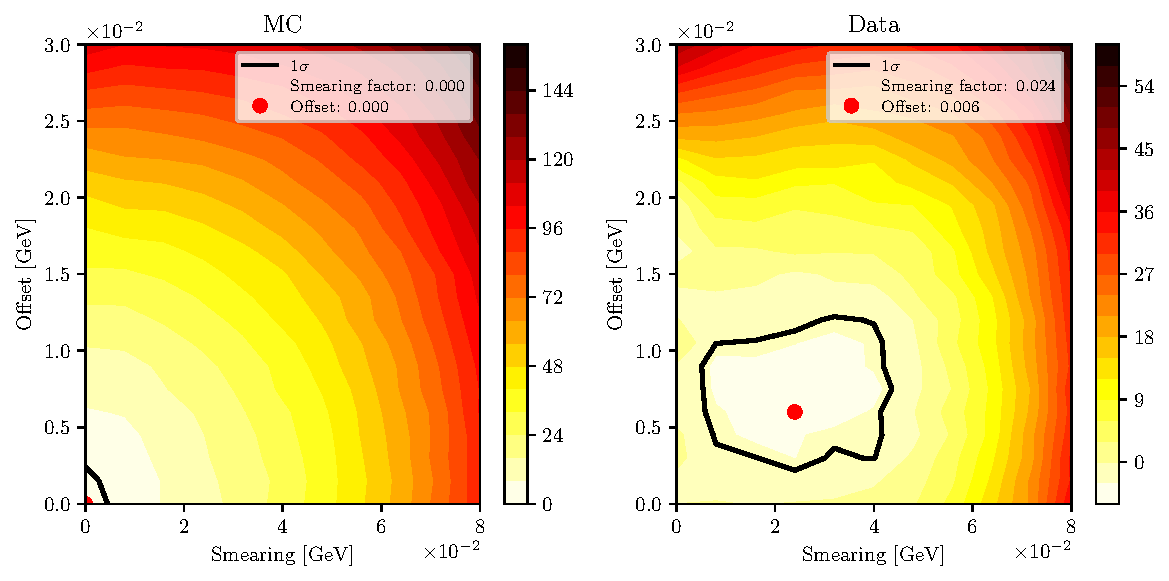
\includegraphics[width=\linewidth]{fig/smearing_offset}
	\caption{Likelihood ratio test of an additional smearing and offset parameter to MC (left) and data (right).}
	\label{fig:smearing_offset}
\end{figure}


\subsection{Signal Fit}\label{sec:templates-in-signal-fits}
The motivation for the choice of signal fit templates comes from Figure \ref{fig:sig_bkg_all_after}. The following histogram templates were defined
\begin{itemize}
	\item signal template,
	\item $q \bar q$ template,
	\item a series of well defined templates from $B \bar B$ background:
	\begin{itemize}
		\item $C_0:~B^+ \to \bar{D} {}^0 \ell^+ \nu,~D^0 \to K^-K^+$ (control decay),
		\item $C_1:~B \to \bar{D} {}^* \ell^+ \nu,~D^0 \to K^-K^+$,
		\item $C_2:~B \to \bar{D} {}^{(*)} \ell^+ \nu,~D^0 \to K^-\pi^+$,
		\item $C_3:~B \to \bar{D} {}^{(*)} \ell^+ \nu,~D^0 \to K^-K^+\pi^0,~K^-\pi^+\pi^0$,
		\item $C_4:~B \to \bar{D} {}{(*)} \ell^+ \nu,~D^0 \to K^-\ell^+\nu$,
		\item $C_5:~B^0 \to D^{(*)-} \ell^+ \nu,~D^+ \to K^-K^+\pi^+,~K^-\pi^+\pi^+$,
		\item $C_6:~$ other $B \to \bar D {}^{(*)} \ell^+ \nu$ decays,
	\end{itemize}
	\item remaining $B \bar B$ background template.
\end{itemize}
As mentioned in chapter \ref{sec:background-suppression}, the majority of the background comes from $B \bar B$ events. Various processes ($C_0$ to $C_6$) contribute to this background which are well known and measured, so we make use of these measurements by fixing their yields in MC fits and appropriately constraining them in real data fits. The remaining $B \bar B$ background is merged into a single template. In this case, the shape of all templates is fixed as well, while the yields are floated for all templates except for the constrained background templates. The yield constraints are based on the channels shown in Table \ref{tab:sig_constraint_table} and defined for each template category as 
\begin{equation}
Y_i = \eta_{\mathrm{norm.}} \times \frac{\left(\sum_j N_{ij}\times \rho_{ij} \right)}{\rho_{00}},
\label{eq:sig_fix}
\end{equation}
where $j$ runs over all channels in the category $C_i$ and where $\rho_{ij}$ is defined in Eq. (\ref{eq:br_fix}). The first factor, $\eta_{\mathrm{norm.}}$, serves as a normalization factor in order to scale the number of generated $B \bar B$ events to the number of $B \bar B$ events in measured data. We define it as
\begin{equation}
\eta_{\mathrm{norm.}} = \frac{N_{\mathrm{control}}^D}{N_{\mathrm{control}}^{MC}},
\end{equation}
where $N_{\mathrm{control}}^D$ and $N_{\mathrm{control}}^{MC}$ are control yields in the control fit for data and MC, respectively.

In addition to branching ratio constraints in Table \ref{tab:cs_br_constraint_table}, further constraints are defined in Table \ref{tab:sig_br_constraint_table} due to more decay channels. In case of the category $C_6$, we have no firm handle on the $D$ meson decay, therefore no correction for this branching ratio can be introduced, so we set a correction factor of $1$ with a $100\%$ error for the $D$ meson decay branching ratio. As most of the correction factors used for constraints have deviations (including the errors) from nominal values well below $100\%$ this value is very conservative.


\begin{table}[H]
	\centering
	\begin{tabular}{|l|l|l|l|l|}
		\hline
		Category & Channel & $B$ Decay Mode & $D$ Decay Mode & Expected MC Yield \\
		\hline
		
		$C_0$ & $N_{00}$ &  $B^+ \to \bar D {}^{0} \ell^+ \nu$ & $D^0 \to K^-K^+$ & $44\pm7$\\
		\hline
		\hline
		
		\multirow{2}{*}{$C_1$} & $N_{10}$ & $B^+ \to \bar D {}^{*0} \ell^+ \nu$ & $D^0 \to K^-K^+$ & $53\pm7$\\
		\cline{2-5}     
		& $N_{11}$ & $B^0 \to D {}^{*-} \ell^+ \nu$  & $D^0 \to K^-K^+$ & $6\pm2$\\
		\hline
		\hline
		
		\multirow{3}{*}{$C_2$} & $N_{20}$ & $B^+ \to \bar D {}^{0} \ell^+ \nu$ & $D^0 \to K^-\pi^+$ & $23\pm5$\\
		\cline{2-5}     
		& $N_{21}$ & $B^+ \to \bar D {}^{*0} \ell^+ \nu$  & $D^0 \to K^-\pi^+$ & $41\pm6$\\
		\cline{2-5}     
		& $N_{22}$ & $B^0 \to D {}^{*-} \ell^+ \nu$  & $D^0 \to K^-\pi^+$ & $6\pm2$\\
		\hline
		\hline
		
		\multirow{6}{*}{$C_3$} & $N_{30}$ & $B^+ \to \bar D {}^{0} \ell^+ \nu$ & $D^0 \to K^-K^+\pi^0$ & $103\pm10$\\
		\cline{2-5}     
		& $N_{31}$ & $B^+ \to \bar D {}^{0} \ell^+ \nu$ & $D^0 \to K^-\pi^+\pi^0$ & $211\pm15$\\
		\cline{2-5}     
		& $N_{32}$ & $B^+ \to \bar D {}^{*0} \ell^+ \nu$ & $D^0 \to K^-K^+\pi^0$ & $135\pm12$\\
		\cline{2-5}
		& $N_{33}$ & $B^+ \to \bar D {}^{*0} \ell^+ \nu$ & $D^0 \to K^-\pi^+\pi^0$ & $267\pm16$\\
		\cline{2-5}
		& $N_{34}$ & $B^0 \to D {}^{*-} \ell^+ \nu$ & $D^0 \to K^-K^+\pi^0$ & $19\pm4$\\
		\cline{2-5}
		& $N_{35}$ & $B^0 \to D {}^{*-} \ell^+ \nu$ & $D^0 \to K^-\pi^+\pi^0$ & $36\pm6$\\
		\hline
		\hline    
		
		\multirow{6}{*}{$C_4$} & $N_{40}$ & $B^+ \to \bar D {}^{0} \ell^+ \nu$ & $D^0 \to K^-e^+\nu$ & $48\pm7$\\
		\cline{2-5}     
		& $N_{41}$ & $B^+ \to \bar D {}^{0} \ell^+ \nu$ & $D^0 \to K^-\mu^+\nu$ & $7\pm3$\\
		\cline{2-5}     
		& $N_{42}$ & $B^+ \to \bar D {}^{*0} \ell^+ \nu$ & $D^0 \to K^-e^+\nu$ & $98\pm10$\\
		\cline{2-5}
		& $N_{43}$ & $B^+ \to \bar D {}^{*0} \ell^+ \nu$ & $D^0 \to K^-\mu^+\nu$ & $10\pm3$\\
		\cline{2-5}
		& $N_{44}$ & $B^0 \to D {}^{*-} \ell^+ \nu$ & $D^0 \to K^-e^+\nu$ & $14\pm4$\\
		\cline{2-5}
		& $N_{45}$ & $B^0 \to D {}^{*-} \ell^+ \nu$ & $D^0 \to K^-\mu^+\nu$ & $3\pm2$\\
		\hline
		\hline    
		
		\multirow{4}{*}{$C_5$} & $N_{50}$ & $B^0 \to D {}^{-} \ell^+ \nu$ & $D^+ \to K^-K^+\pi^+$ & $103\pm10$\\
		\cline{2-5}     
		& $N_{51}$ & $B^0 \to D {}^{-} \ell^+ \nu$ & $D^+ \to K^-\pi^+\pi^+$ & $63\pm8$\\
		\cline{2-5}     
		& $N_{52}$ & $B^0 \to D {}^{*-} \ell^+ \nu$ & $D^+ \to K^-K^+\pi^+$ & $31\pm6$\\
		\cline{2-5}
		& $N_{53}$ & $B^0 \to D {}^{*-} \ell^+ \nu$ & $D^+ \to K^-\pi^+\pi^+$ & $21\pm5$\\
		\hline
		\hline
		
		\multirow{4}{*}{$C_6$} & $N_{60}$ & $B^+ \to \bar D {}^{0} \ell^+ \nu$ & \multirow{4}{*}{} & $69\pm8$\\
		\cline{2-3}     
		\cline{5-5}     
		& $N_{61}$ & $B^+ \to \bar D {}^{*0} \ell^+ \nu$ & Other $D^0$ and $D^+$ & $95\pm10$\\
		\cline{2-3}     
		\cline{5-5}
		& $N_{62}$ & $B^0 \to D {}^{-} \ell^+ \nu$ & decays & $63\pm8$\\
		\cline{2-3}     
		\cline{5-5}
		& $N_{63}$ & $B^0 \to D {}^{*-} \ell^+ \nu$ &  & $36\pm6$\\
		\hline
		
	\end{tabular}
	\caption{}
	\label{tab:sig_constraint_table}
\end{table}

\begin{table}[H]
	\centering
	\begin{tabular}{|c|l|l|l|c|c|}
		\hline
		$\mathcal{B}$ ID & Decay & $\mathcal{B}_{GEN}$ & $\mathcal{B}_{PDG}$ & $\rho$ & Reference \\ 
		\hline
		5 &	$D^0 \to K^-\pi^+$ & $3.82\E{-2}$ & $(3.89\pm0.04)\E{-2}$ & $1.02 \pm 0.01$ & \multirow{7}{*}{ \cite{tanabashi2018review}} \\
		\cline{1-5}
		6 & $D^0 \to K^-K^+\pi^0$ & $2.36\E{-3}$ & $(3.37\pm0.15)\E{-3}$ & $1.43 \pm 0.06$ & \\
		\cline{1-5}
		7 & $D^0 \to K^-\pi^+\pi^0$ & $13.08\E{-2}$ & $(14.2\pm0.5)\E{-2}$ & $1.09 \pm 0.04$ &  \\
		\cline{1-5}
		8 & $D^0 \to K^-e^+\nu$ & $3.41\E{-2}$ & $(3.53\pm0.028)\E{-2}$ & $1.04 \pm 0.01$ &  \\
		\cline{1-5}
		9 & $D^0 \to K^-\mu^+\nu$ & $3.41\E{-2}$ & $(3.31\pm0.13)\E{-2}$ & $0.97 \pm 0.04$ &  \\
		\cline{1-5}
		10 & $D^+ \to K^-K^+\pi^+$ & $9.06\E{-3}$ & $(9.51\pm0.34)\E{-3}$ & $1.05 \pm 0.04$ &  \\
		\cline{1-5}
		11 & $D^+ \to K^-\pi^+\pi^+$ & $9.51\E{-2}$ & $(8.98\pm0.28)\E{-2}$ & $0.94 \pm 0.03$ &  \\
		\hline
	\end{tabular}
	\caption{Additional MC and measured values of $D$ meson branching ratios along with the calculated correction factors used for constraining the signal fit.}
	\label{tab:sig_br_constraint_table}
\end{table}

\section{Adaptive Binning Algorithm}\label{sec:adaptive-binning-algorithm}

The fit templates contain areas of low statistics, which are populated with bins with zero content. This is a direct consequence of having a finite MC sample and represent a liability in ML fits. Due to low statistics in the edge regions, the locations of these empty bins can vary for the templates and the fitted sample. A problem occurs if all templates have an empty bin where the fitted sample does not. In the scope of ML fits, this effectively means that there are entries in bins where the probability of having them is $0$. We will call such bins \textit{problematic} because in these cases the fit does not converge.

The ideal solution for this problem would be to increase the MC statistics. Since this is not an option, we pursue other solutions, such as decreasing the number of bins. While this solves the problem, the drawback of it is a decrease in the template resolution in densely populated regions, where good resolution is most needed. The optimal solution here seems to be a choice of variable bins, with fine binning in the densely populated regions and larger bins in the regions with low statistics.

We have devised an algorithm, which compares the templates and the fitted sample, and defines a variable binning so that there are no more problematic bins in the end. Figure \ref{fig:adapt} shows an example of how the procedure works. The algorithm takes an argument for the initial number of uniform bins in each dimension and does the following
\begin{enumerate}
	\item define uniform binning in both dimensions with the provided argument,
	\item create a 2D histogram from MC templates with expected yields,
	\item define an \textit{optimal} region, where most of the 2D integral is contained and where all bins have a non-zero content (this region does not change throughout the process),
	\item compare the histograms for the expected and the fitted sample, find the problematic bins,
	\item loop until all problematic bins disappear
	\begin{enumerate}
		\item find the problematic bin, which is nearest to the maximum bin,
		\item change the binning from $N$ to $N-1$ from that bin and in the direction away from the maximum bin.
	\end{enumerate}
\end{enumerate}

\begin{figure}[H]
	\centering
	\captionsetup{width=0.8\linewidth}
	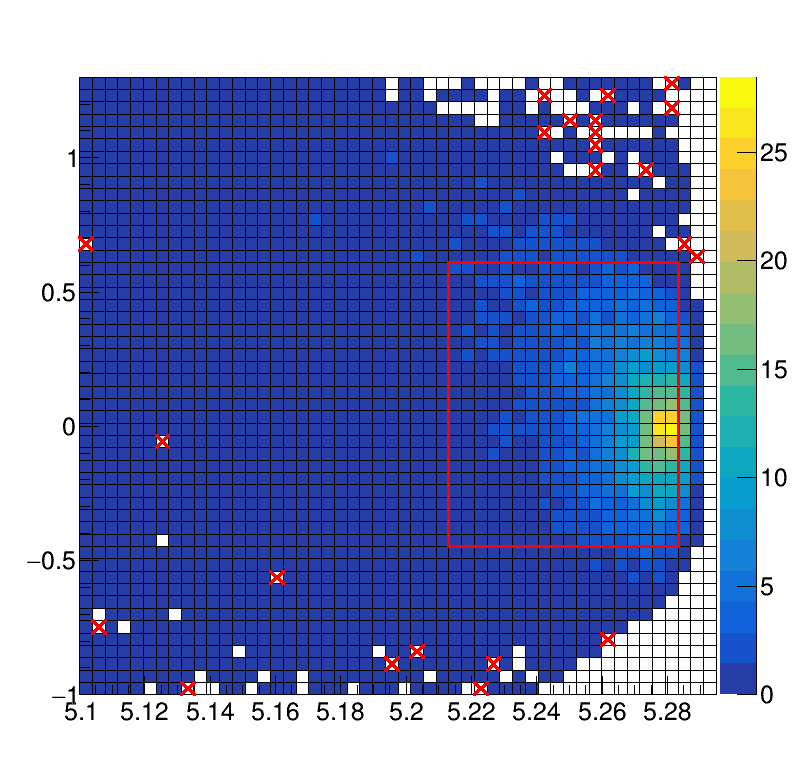
\includegraphics[width=0.49\linewidth]{fig/adaptive_1}
	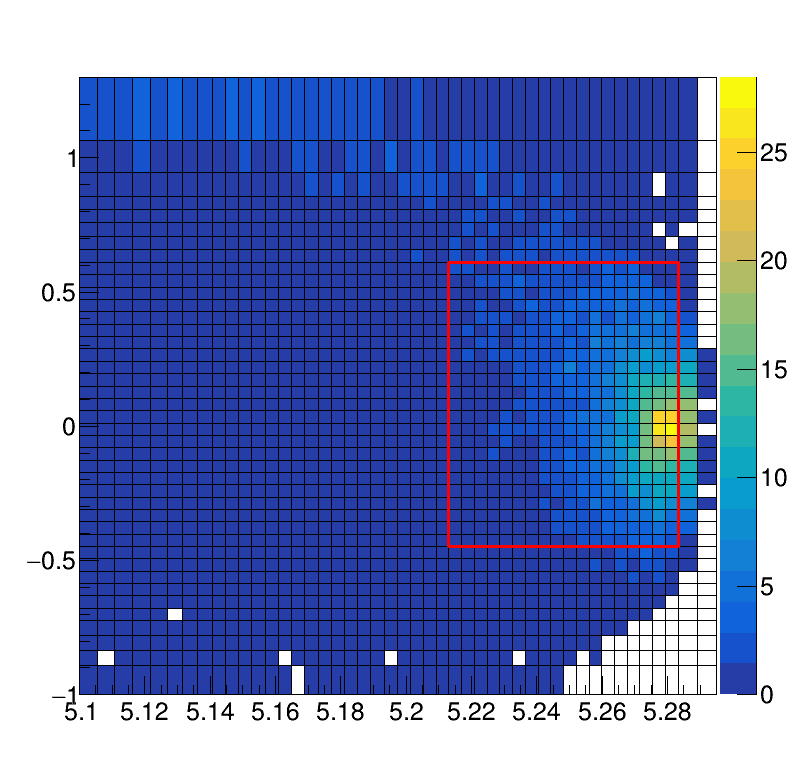
\includegraphics[width=0.49\linewidth]{fig/adaptive_15}
	\caption{Steps taken in the adaptive binning algorithm. Left image shows the initial 2D histogram with the defined optimal region and the problematic bins, the right image shows the final binning with the unchanged optimal region, while the problematic bins are gone due to the new binning choice.}
	\label{fig:adapt}
\end{figure}

An additional problem occurs in the plotting of the fitted templates and the sample with variable binning. It would seem that RooFit does not take the bin widths into account when plotting, while everything works as expected for the fit itself. This was bypassed by extracting the fitted yields and applying them to templates and samples with uniform binning, which were then used for drawing.

\section{Toy MC Experiments}

For the chosen final selection and fit procedure, toy MC pseudo-experiments were performed in order to confirm the behavior of the fit setup. The fit behavior is also checked as a function of the signal yield in the form of a linearity test. A detailed description of toy MC experiments is written in this section.

With toy MC experiments in this section, we study the yields, errors and the pulls of the signal fit by generating our own pseudo data sets, according to the MC. This significantly reduces the time we would need to produce the data sets in the standard way, while still reliably describing the underlying physics behind the pseudo data set. All available MC was used for pseudo data set generation as well as creating templates. 

\subsection{Pseudo Experiment: Expected Signal Yield}

We constructed $3\E{3}$ pseudo data sets, where each data set was generated with the expected amount of each template category, distributed according to the Poisson distribution. All fits were performed with the optimal initial uniform binning of $19 \times 19$ bins in \vars.

Figure \ref{fig:toyMC} shows distributions of the fit yields, errors and the pull distribution of all pseudo fits. The fits seem to be under control, although there is a slight bias present in the negative direction, which can also be seen in the pull distribution plot. The latter follows a normal distribution with a mean of $(-0.11\pm0.02)$ and standard deviation of $(1.01\pm0.01)$. The mean ($\bar X$) and the standard deviation $(S)$ were calculated in the usual way, while their errors $\sigma_{\bar X}$ and $\sigma_S$ were calculated as \cite{ahn2003standard}
\begin{equation}
\sigma_{\bar X} = \frac{S}{\sqrt{N}},\quad \sigma_{S} = \frac{S}{\sqrt{2(N-1)}},
\end{equation}
where $N$ is the number of performed measurements.

\begin{figure}[H]
	\centering
	\captionsetup{width=0.8\linewidth}
	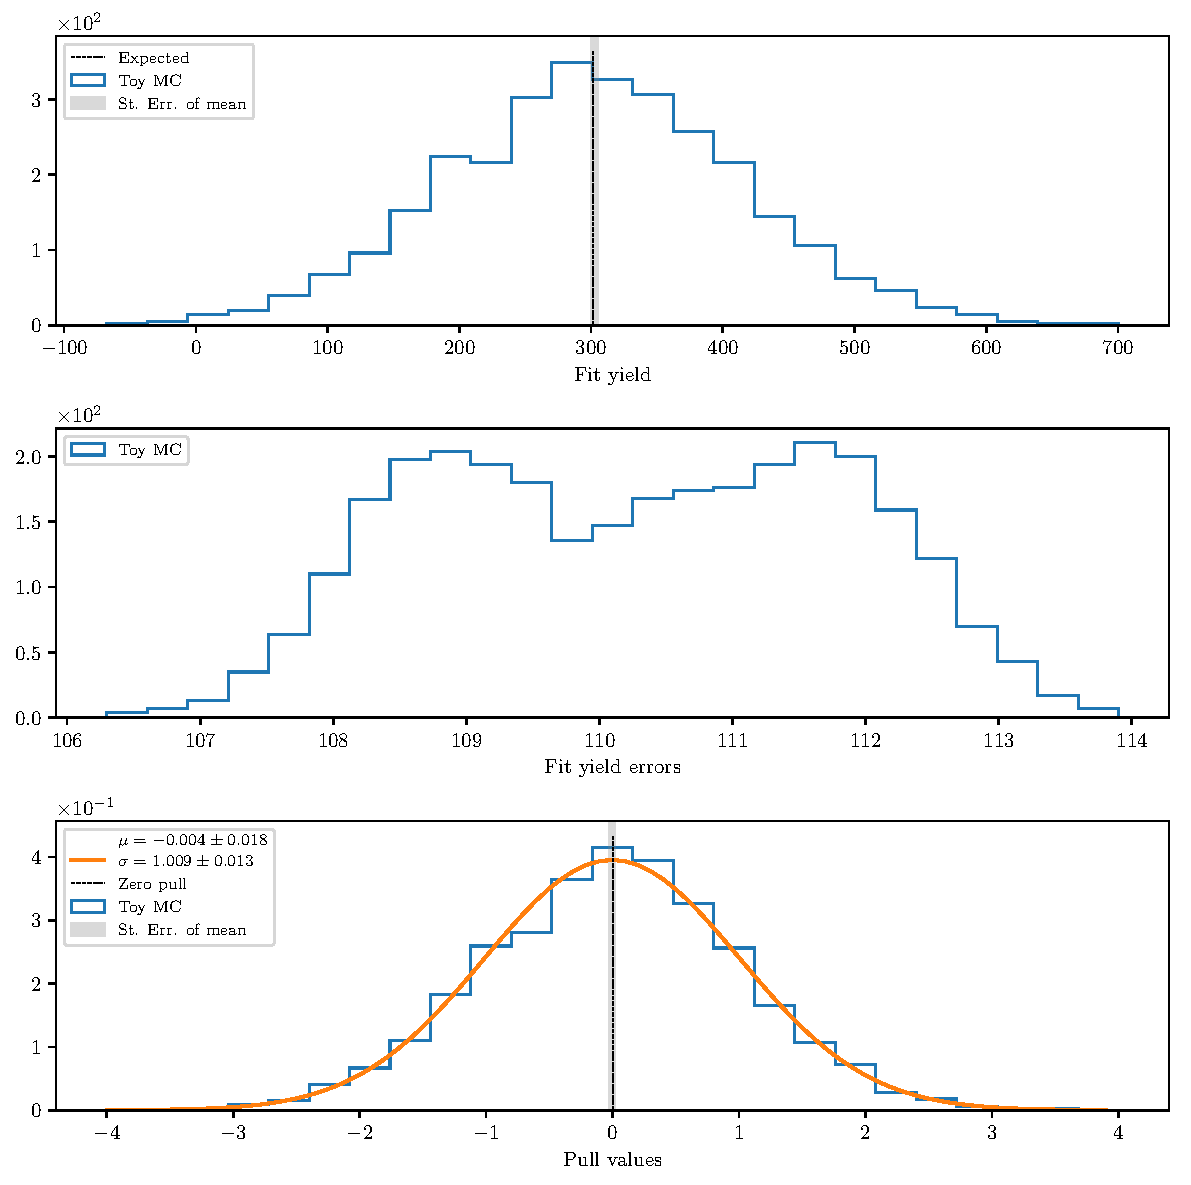
\includegraphics[width=\linewidth]{fig/toyMC}
	\caption{Toy MC fits of pseudo data showing the fit yield (top), fit errors (center) and the pull distribution of the fits (bottom).}
	\label{fig:toyMC}
\end{figure}

\subsection{Pseudo Experiment: Linearity Test}
\label{sec:pseudo-experiment-linearity-test}
Linearity test is used for determining the sensitivity of the fit to the amount of signal in the fitted sample. Since this is the first measurement of this decay channel, MC modeling is not reliable and could be very different from reality, so we need to perform this test in order to determine our sensitivity to smaller, as well as larger amounts of expected signal.

The pseudo data sets are generated in the same way as in the previous subsection, with the exception of signal, which is generated in various amounts. $50$ steps from $[0.1,~10]$ in the logarithmic scale are taken for fractions of signal amount and for each fraction we generate 500 pseudo data sets according to Poisson statistics.

Figure \ref{fig:lin_test} shows the difference between mean fit yield and the expected yield, mean pull and the mean significance at each signal fraction value. The expected MC result lies at the fraction value $10^0 = 1$. The plots show no significant bias with respect to the signal fraction, while the pulls seem to be described by the normal distributions throughout the fraction range. At expected value, we are at about $3.58\sigma$ significance.

\begin{figure}[H]
	\centering
	\captionsetup{width=0.8\linewidth}
	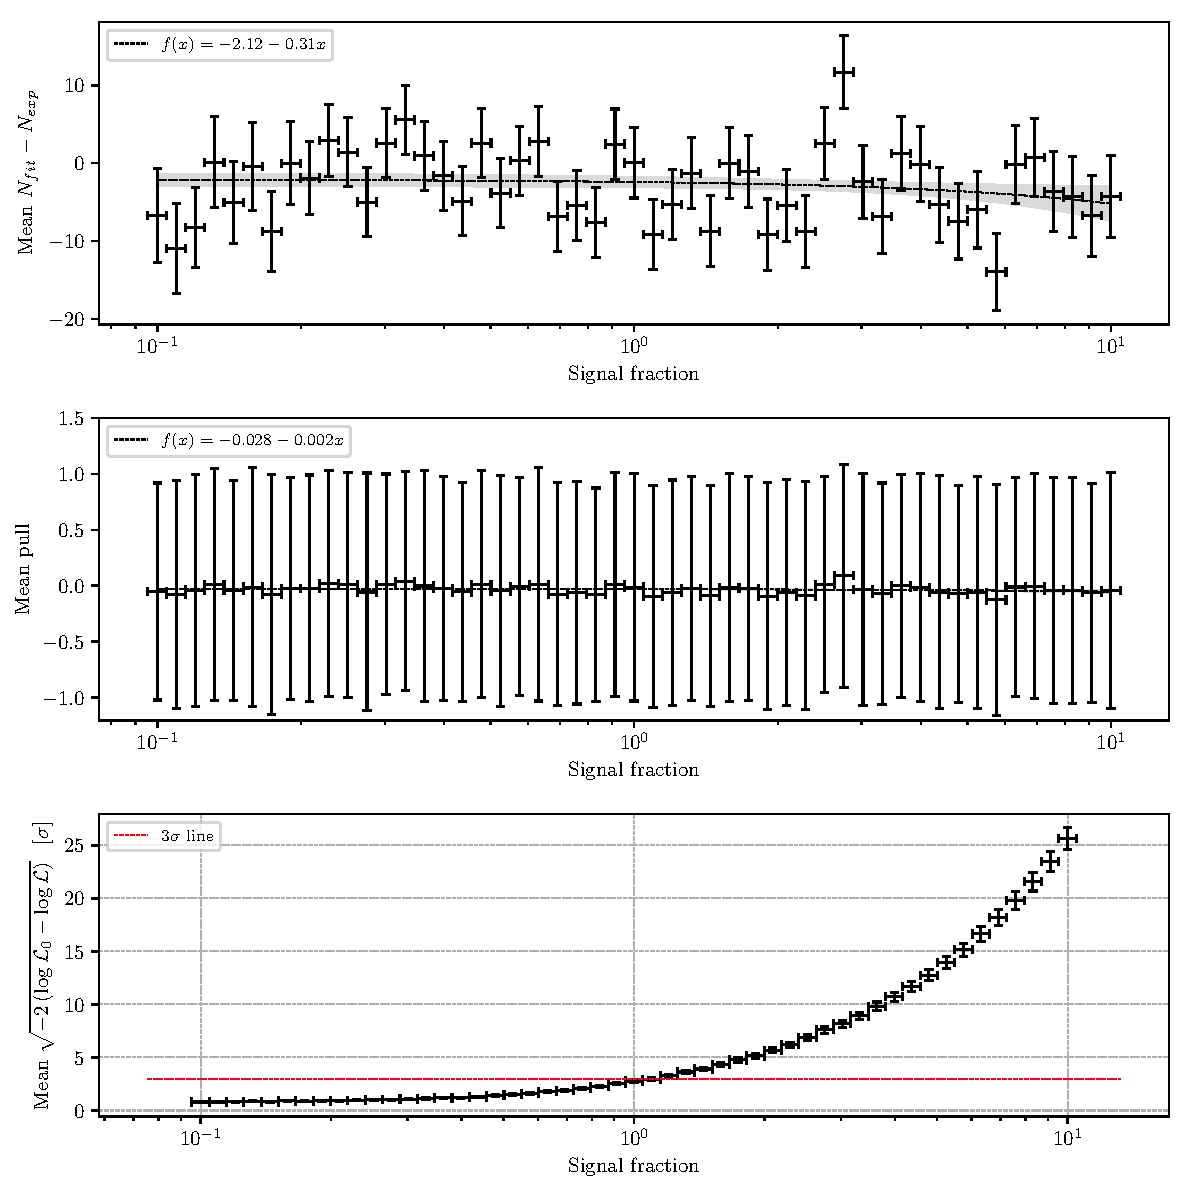
\includegraphics[width=\linewidth]{fig/lin_test}
	\caption{Mean fit yield and expected yield difference (top), mean pull (center) and mean significance (bottom) as a function of signal fraction.}
	\label{fig:lin_test}
\end{figure}


\section{Fit Results}
In this section, we present the first results of signal and control fits on MC as well as data, along with the control decay branching ratio measurement. We also show results of the signal fit on MC and data.

\subsection{Signal MC Fit Results}\label{sec:signal-mc-fit-results}

With the signal fit setup described in section \ref{sec:templates-in-signal-fits}, we proceed to fit the 10 streams of MC. To compare both methods of $B \bar B$ bar suppression, two different samples were prepared and used in the fit. Since the choice of initial uniform binning is not obvious, we perform fits to all streams of MC for each initial binning choice in the range $N\times N,~N\in[4,30]$. Figure \ref{fig:sig_binning} shows the expected yield differences, pulls and fit significances for both final samples for each binning case. The difference between fitted an expected signal yield should be equal to 0 to ensure no bias is present in the fit, while the average pull distribution for each bin case should have a central value at 0, with a width of 1.  While both fit results seem to have no significant bias with respect to the binning choice, the pull distribution seems to be closer to the normal distribution. The uBDT classifier fit setup outperforms the standard BDT fit setup in terms of significance by $1\sigma$. This determines our choice of the final selection. The binning in \vars~is chosen at the plateau of the significance, where no significant bias is present and is somewhere in the region of $20$ bins in each dimension.

\begin{figure}[H]
	\centering
	\captionsetup{width=0.8\linewidth}
	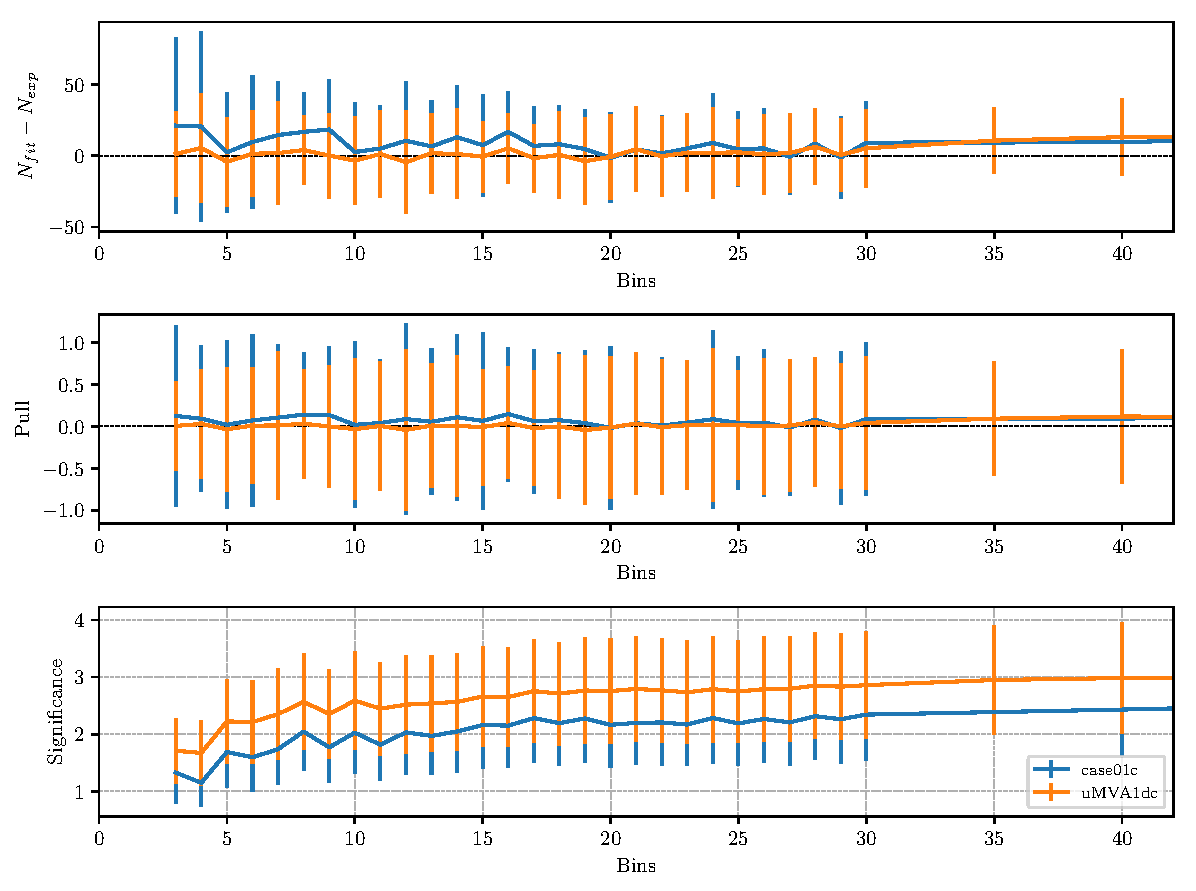
\includegraphics[width=\linewidth]{fig/sig_binning}
	\caption{Fitted yield and expected yield difference (top), pulls (center) and fit significance (bottom) as a function of binning in \vars~for the final sample, optimized with the standard BDT classifier (blue) and the uBDT classifier (orange).}
	\label{fig:sig_binning}
\end{figure}

For the chosen binning of $19 \times 19$ in \vars~we perform the 10 stream MC fits, where an average stream fit is shown in Figure \ref{fig:sig_streamfit}, while all fit results are shown in Figure \ref{fig:sig_global}. All stream fit results were fitted with a 0th-degree polynomial. The global result seems to describe the expected value in a precise manner, with the bias much smaller than the average statistical error. The normalized $\chi^2$ value with $10-1=9$ degrees of freedom of the global fit is $\chi^2_9 = 0.98$, while the average significance of the fits is around $3.56 \sigma$.

\begin{figure}[H]
	\centering
	\captionsetup{width=0.8\linewidth}
	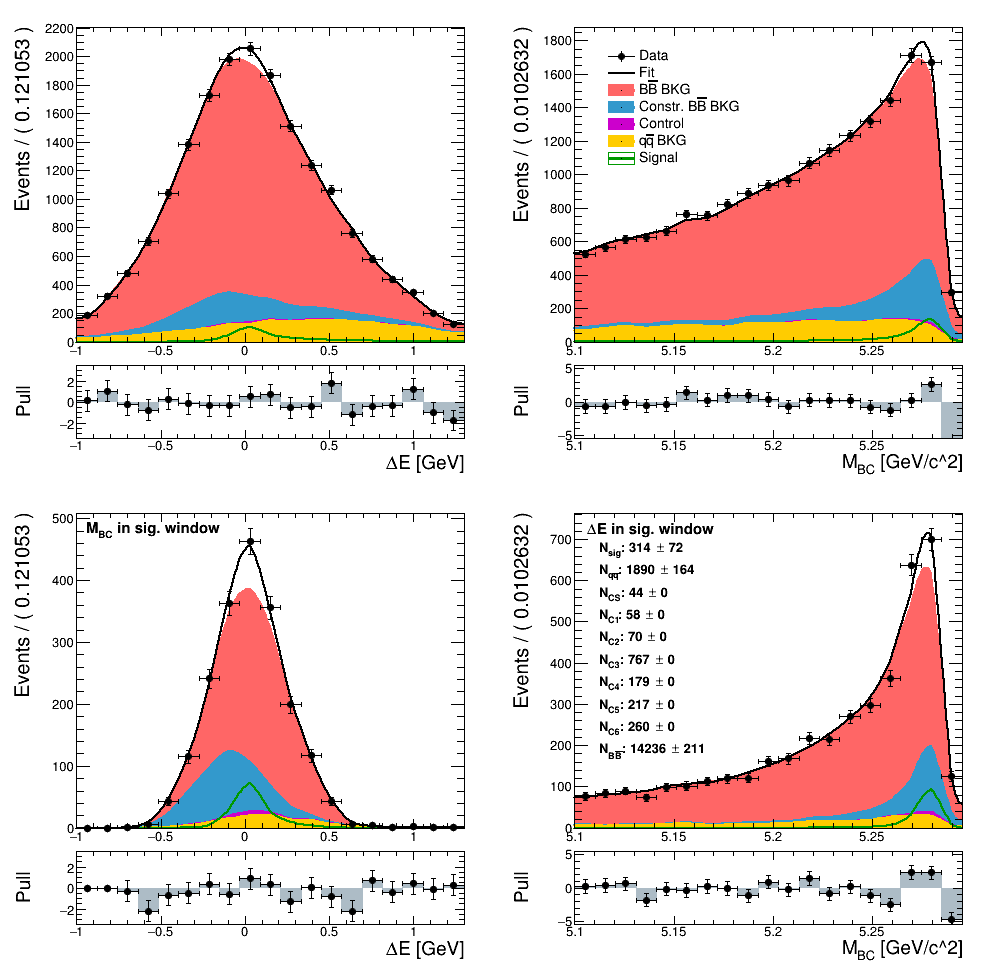
\includegraphics[width=\linewidth]{fig/sig_fit_mc}
	\caption{An example fit to one stream of MC. Left column shows the $M_{BC}$ and the right column shows the $\Delta E$ distribution of the full fitted sample in the full fit region (top) and the signal region (bottom).}
	\label{fig:sig_streamfit}
\end{figure}

\begin{figure}[H]
	\centering
	\captionsetup{width=0.8\linewidth}
	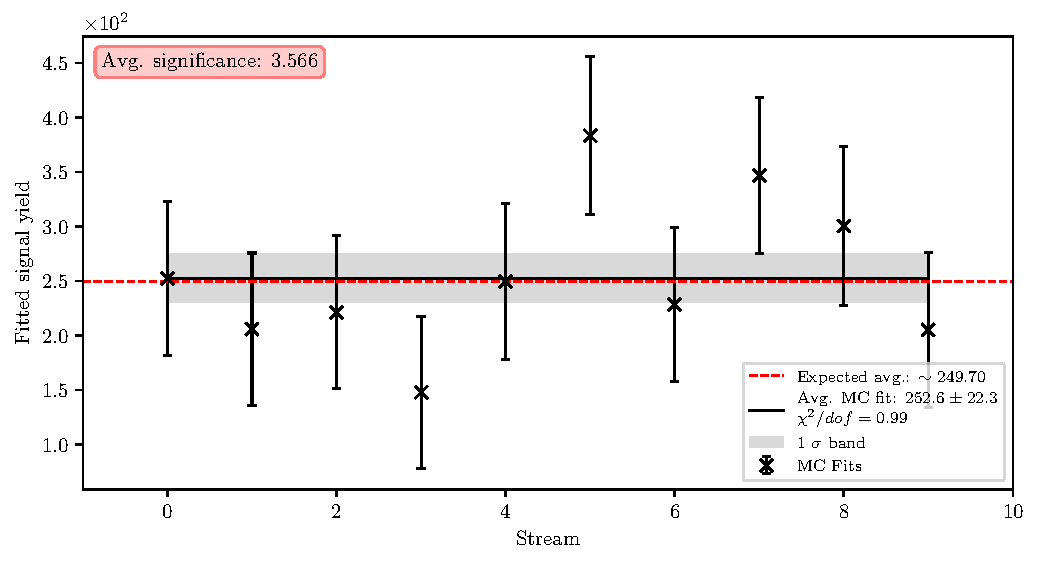
\includegraphics[width=\linewidth]{fig/sig_global_mc}
	\caption{Fits to all 10 streams of MC and the global fit with a zero degree polynomial. The red line shows the mean value of the global fit and the gray band shows the $1\sigma$ confidence interval.}
	\label{fig:sig_global}
\end{figure}

\subsection{Control Fit Result}
With the control fit setup described in section \ref{sec:control-fit}, we proceed to fit the control sample after the final selection for 10 streams of MC and 1 stream of data. An average MC stream fit is shown in Figure \ref{fig:cs_fit_mc} for MC and Figure \ref{fig:cs_fit_data} for data, while all fit results are shown in Figure \ref{fig:cs_global}, where all streams of MC are fitted with a 0th degree polynomial. The control fit results for split and joined lepton modes are shown in Table \ref{tab:cs_fit_yield}.
\begin{table}[H]
	\centering
	\begin{tabular}{|l|c|c|}
		\hline
		& $N^{MC}$ & $N^{\mathrm{data}}$ \\
		\hline
		$\ell = e$ or $\mu$ & $1180 \pm 11$ & $1192 \pm 44$\\
		\hline
		$\ell = e$ & $590 \pm 9$ & $588 \pm 28$ \\
		\hline
		$\ell = \mu$ & $591 \pm 7$ & $610 \pm 30$\\
		\hline
	\end{tabular}
	\caption{Control sample fit results for MC and data for various lepton final state modes.}
	\label{tab:cs_fit_yield}
\end{table}

\begin{figure}[H]
	\centering
	\captionsetup{width=0.8\linewidth}
	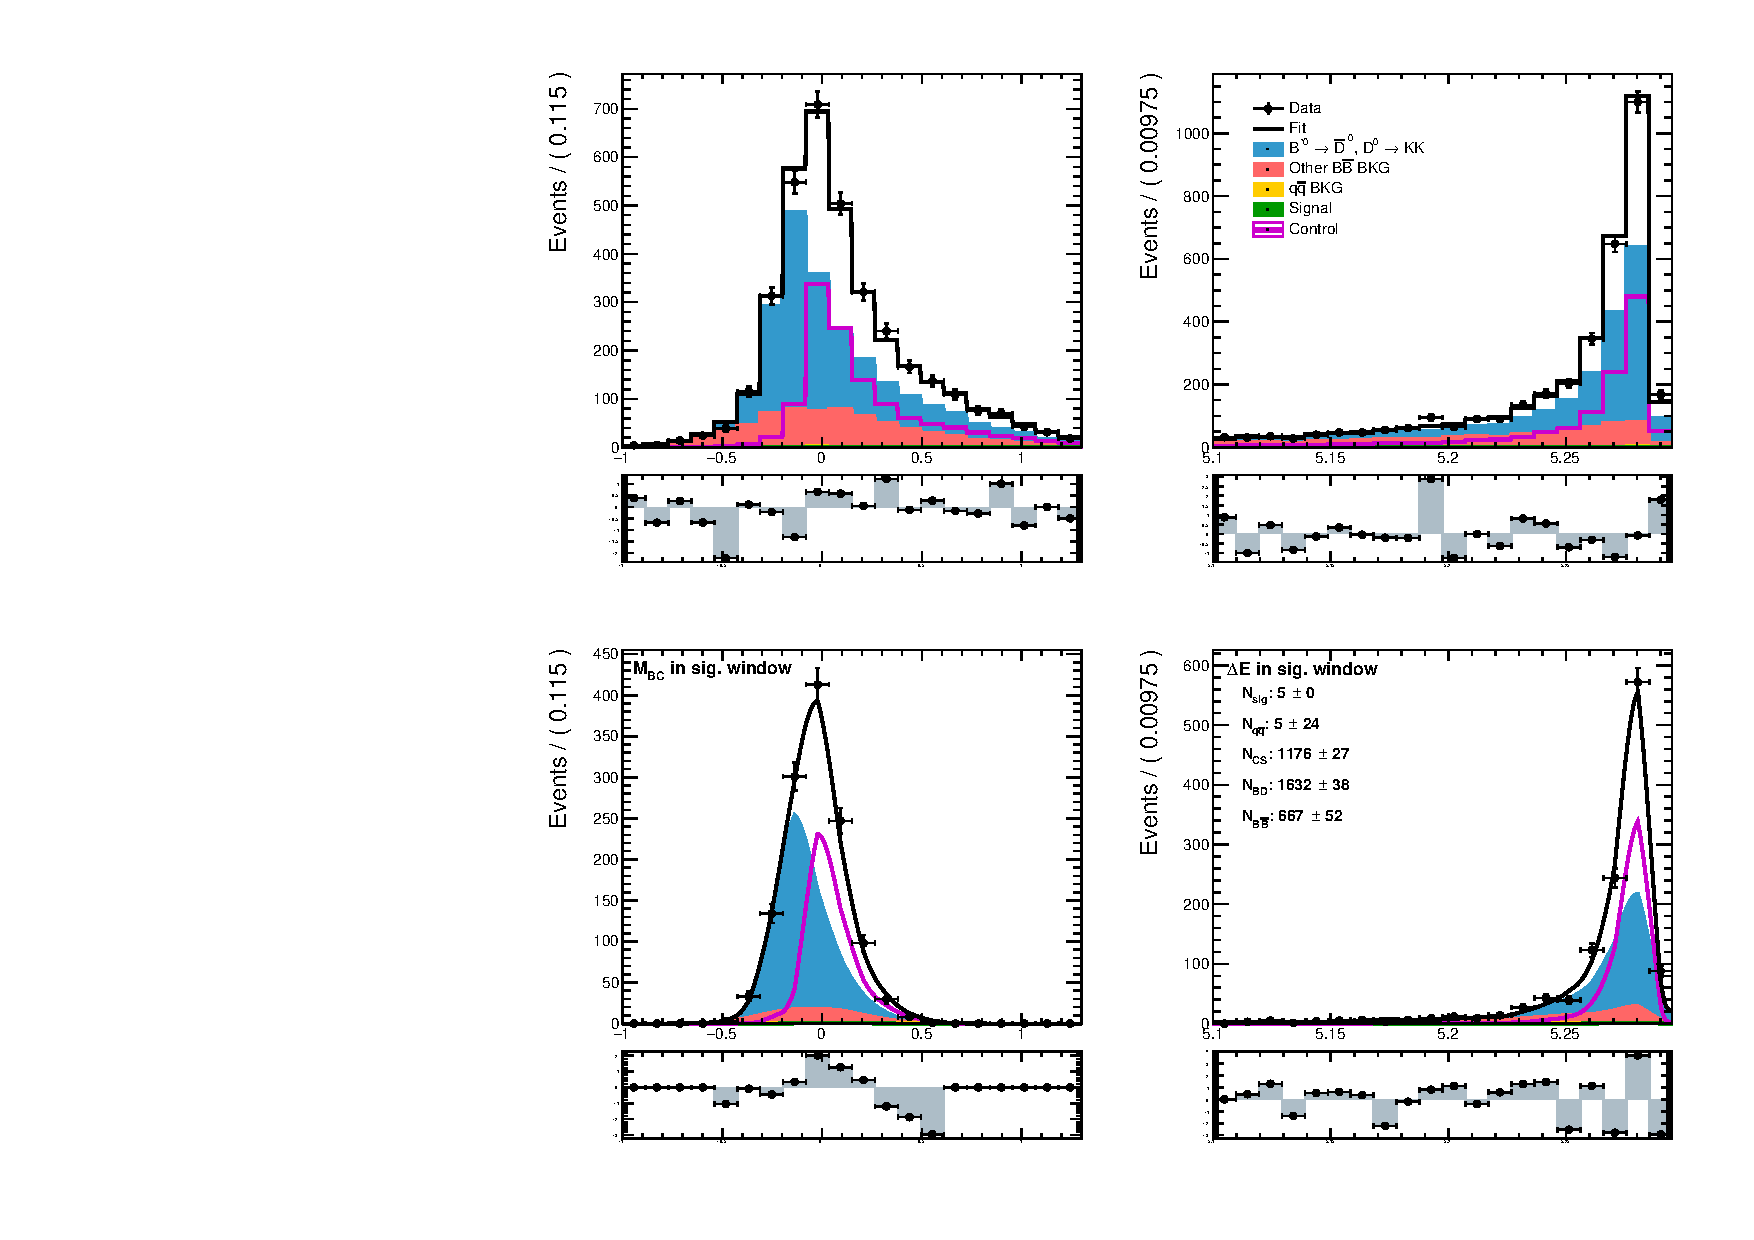
\includegraphics[width=\linewidth]{fig/cs_fit_mc}
	\caption{Control fit result on stream 9 of MC. Left column shows the $M_{BC}$ and the right column shows the $\Delta E$ distribution in the full fit window (top) and the signal window (bottom).}
	\label{fig:cs_fit_mc}
\end{figure}

\begin{figure}[H]
	\centering
	\captionsetup{width=0.8\linewidth}
	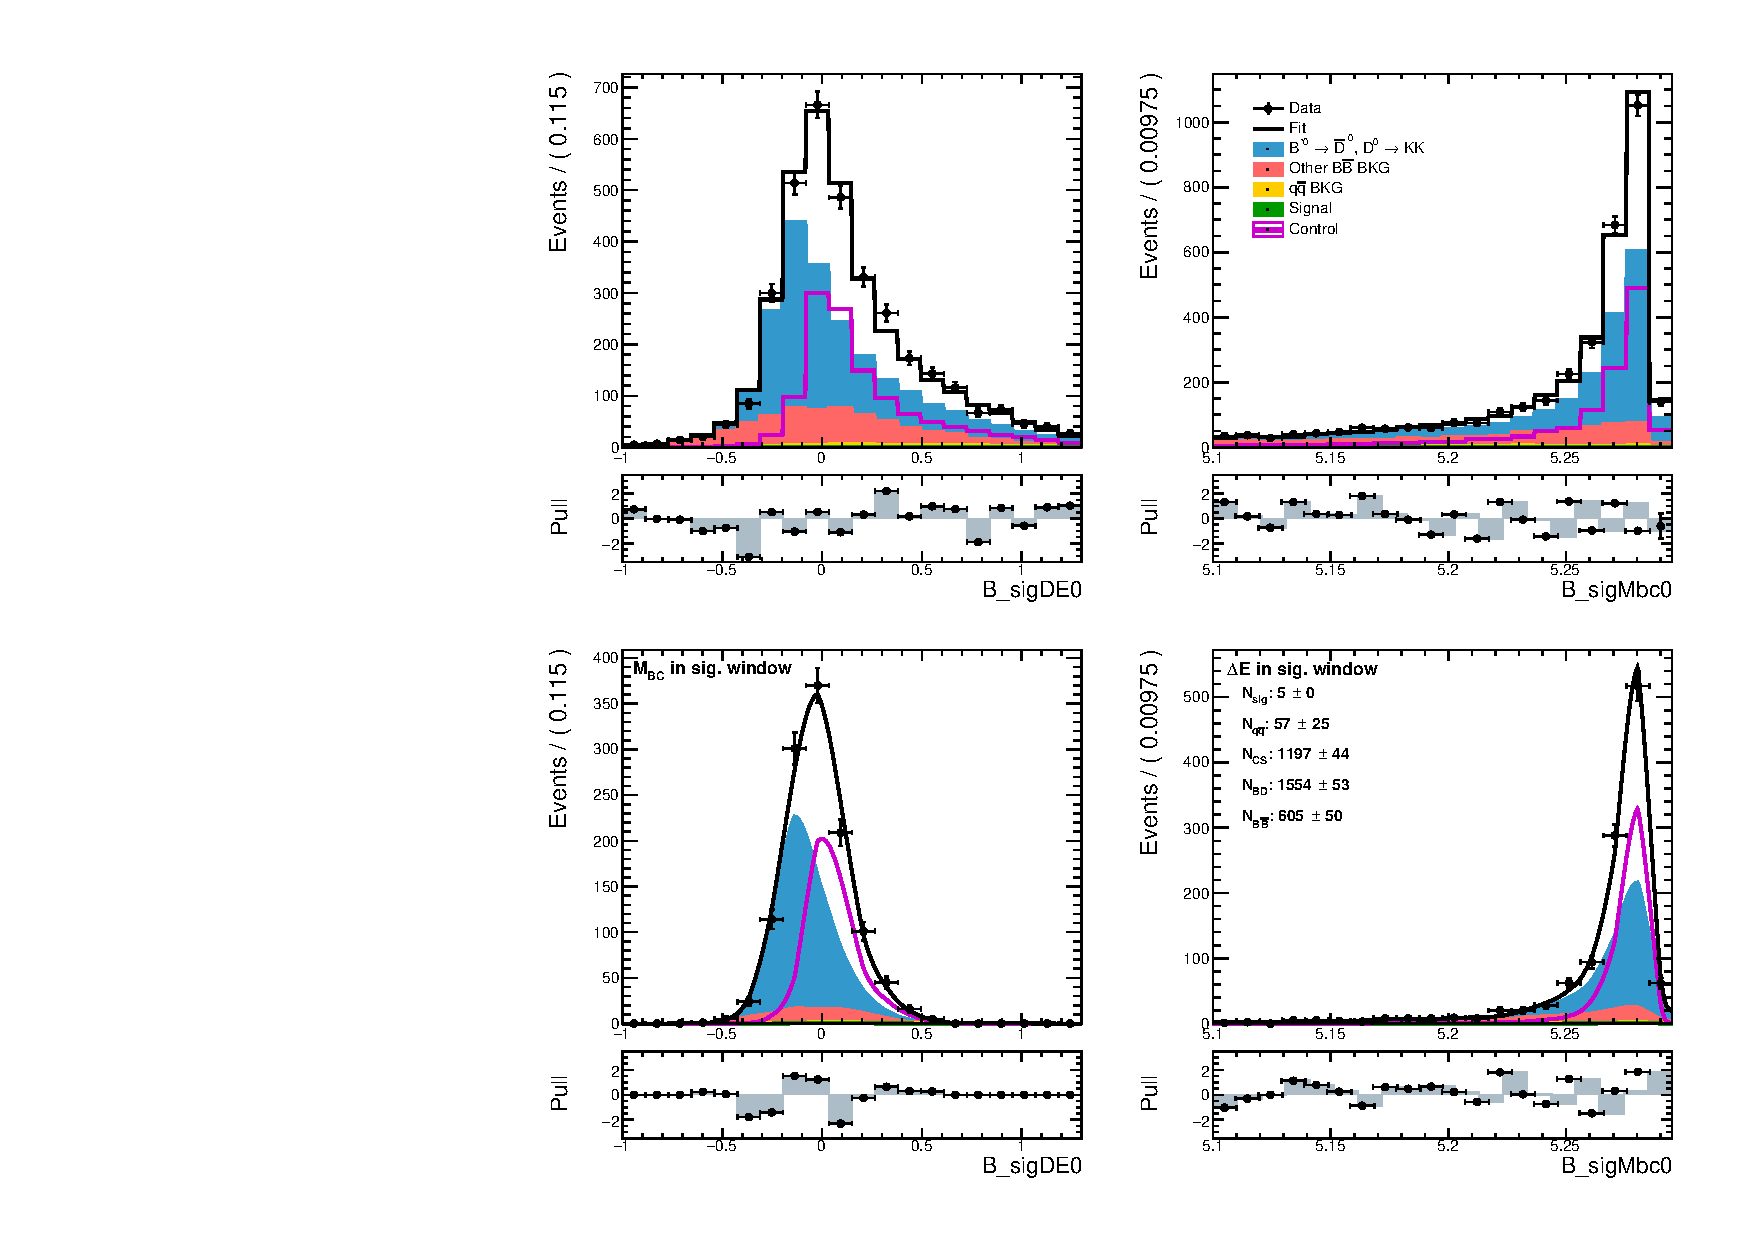
\includegraphics[width=\linewidth]{fig/cs_fit_data}
	\caption{Control fit result on real data. Left column shows the $M_{BC}$ and the right column shows the $\Delta E$ distribution in the full fit window (top) and the signal window (bottom).}
	\label{fig:cs_fit_data}
\end{figure}

\begin{figure}[H]
	\centering
	\captionsetup{width=0.8\linewidth}
	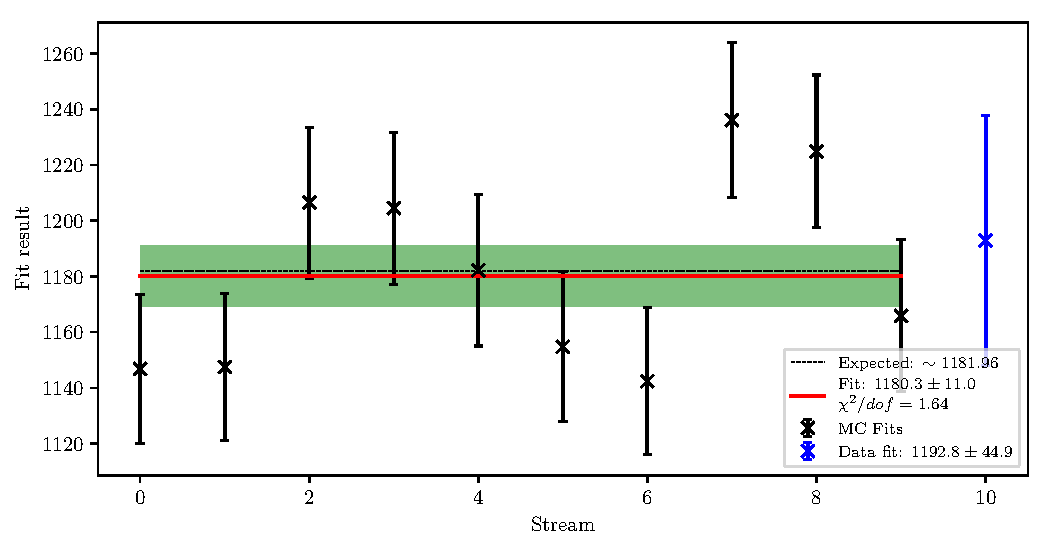
\includegraphics[width=\linewidth]{fig/cs_global}
	\caption{Control fit to data and to all 10 streams of MC. The red line shows the mean value of the global MC fit with a 0th degree polynomial. The gray band shows the $1\sigma$ confidence interval around the global MC fit.}
	\label{fig:cs_global}
\end{figure}


\subsection{Branching Ratio Measurement for Control Decay}

After acquiring the fit results on MC and data, we are able to determine the branching ratio of the control decay, which is defined as
\begin{align}
\mathcal{B}^{MC}_{\mathrm{control}} &= \frac{N^{\mathrm{MC}}_\mathrm{control} \times \epsilon_{MC}}{2N_{B\bar B}^{MC}},\\
\mathcal{B}_{\mathrm{control}} &= \frac{N_\mathrm{control} \times \epsilon_{MC} \times \rho_{PID}}{2N_{B\bar B}},
\label{eq:br_data}
\end{align}
where $N^{\mathrm{MC}}_\mathrm{control}$ and $N_\mathrm{control}$ are yields of the control fit on MC and data, $\epsilon_{MC}$ is the MC efficiency of the control sample, $\rho_{PID}$ the PID correction factor, and $N_{B\bar B}^{MC}$ and $N_{B\bar B}$ are the numbers of $B \bar B$ meson pairs on MC and data, respectively. The factor of 2 in the denominator comes from the fact that there are 2 $B$ mesons in each $B$ meson pair $(\times 1/2)$, where only about $50\%$ of the $B$ meson pairs are charged $B^+B^-$ meson pairs $(\times 2)$, and from the fact that we are interested in the branching ratio to the lepton final state of either $e$ or $\mu$, and not their sum $(\times 1/2)$.

The control sample efficiency was determined on a separate signal MC sample of the control decay, where we generated $5\E{6}$ $B^+ \bar B^-$ pairs, with one $B$ always decaying via $B^+ \to \bar D {}^0 \ell^+ \nu,~D^0 \to K^+K^-$. After applying the final selection, the full and split efficiencies with regard to the lepton final state were determined to be 
\begin{align*}
\epsilon_{MC} &= (8.89\pm 0.04)\E{-3},\\
\epsilon_{MC}^e &= (4.40\pm 0.03)\E{-3},\\
\epsilon_{MC}^\mu &= (4.49\pm 0.03)\E{-3},
\end{align*}
where the efficiency error was estimated based on a formula from \cite{paterno2004calculating}.
\begin{equation*}
\epsilon_{MC} = \frac{1}{N}\sqrt{n(1-\frac{n}{N})},
\end{equation*}
where $n$ is a subset of the full set $N$.

The PID correction factor is obtained by taking into account the known PID efficiency differences between data and MC. It is described in detail in X and is determined to be
\begin{equation*}
\rho_{PID} = 0.99\pm 0.02
\end{equation*}
for the $e$ and $\mu$ mode, as well as both of them together.

The number of $B\bar B$ meson pairs can be counted on MC and has been measured for data by the collaboration. The values are
\begin{align*}
&N_{B\bar B}^{MC} = 765.98\E{6},\\
&N_{B\bar B} = (771.58 \pm 10.56)\E{6}.
\end{align*}

Finally, we can determine the branching ratios based on the calculations in Eq. (\ref{eq:br_data}). The obtained values are shown in Table \ref{tab:br_result} and graphically shown in Figure \ref{fig:br_plot}, along with the MC generated value and the current PDG world average. Both MC and measured determinations of the control decay branching ratio are in agreement with the expected and the world average values. One should note that the black error bars correspond to statistical uncertainty. Of all the systematic uncertainties, only the PID systematics are included in this results. Other contributions of systematics are not included since this measurement is not the goal of our analysis.

\begin{table}[H]
	\centering
	\begin{tabular}{|l|c|c|}
		\hline
		$\mathcal{B}_{PDG}$ & \multicolumn{2}{c|}{$(9.10\pm0.42)\E{-5}$} \\
		\hline
		$\mathcal{B}_{GEN}$ & \multicolumn{2}{c|}{$9.01\E{-5}$} \\
		\hline
		& $\mathcal{B}^{MC}$ & $\mathcal{B}^{\mathrm{data}}$ \\
		\hline
		$\ell = e$ or $\mu$ & $(8.94\pm0.09)\E{-5}$ & $(9.06\pm0.4)\E{-5}$\\
		\hline
		$\ell = e$ & $(9.04\pm0.15)\E{-5}$ & $(9.07\pm0.49)\E{-5}$ \\
		\hline
		$\ell = \mu$ & $(8.85\pm0.12)\E{-5}$ & $(9.12\pm0.50)\E{-5}$\\
		\hline
	\end{tabular}
	\caption{Control sample fit results for MC and data for various lepton final state modes.}
	\label{tab:br_result}
\end{table}

\begin{figure}[H]
	\centering
	\captionsetup{width=0.8\linewidth}
	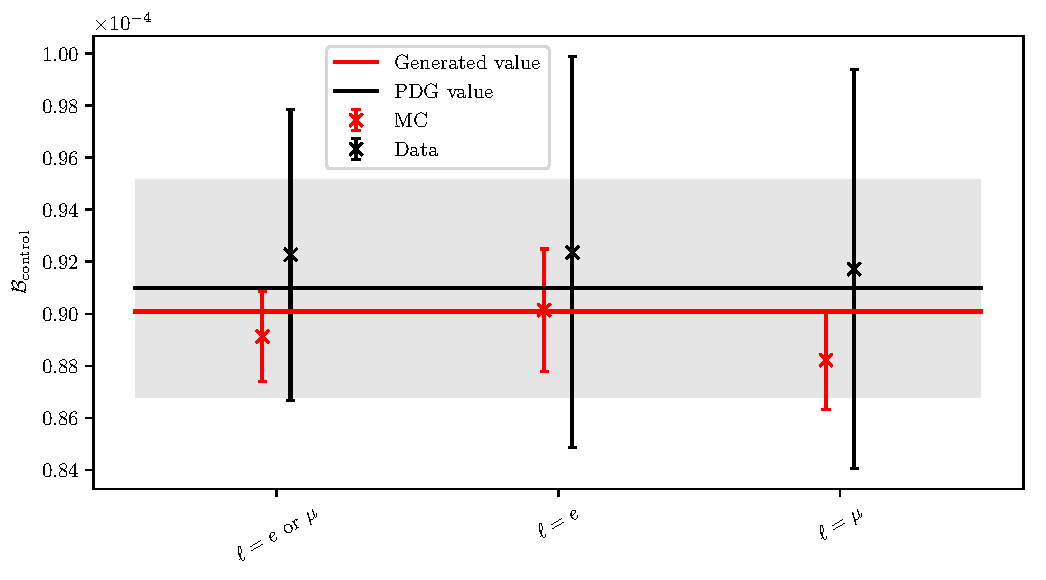
\includegraphics[width=\linewidth]{fig/br_plot}
	\caption{Various branching ratio determinations for the control decay of our analysis.}
	\label{fig:br_plot}
\end{figure}

\subsection{Signal Fit to Data}
Finally, after making sure that the analysis procedure makes sense on the control MC, control data and signal MC sample, we can continue to perform the signal extraction process on the full Belle $\Upsilon(4S)$ data sample. Figure \ref{fig:sig_fit_data} shows the fit result in projections of \vars~ for both fit regions. The extracted signal yield on data as well as the yields of the remaining contributions are shown in Table \ref{tab:sig_yields}. Values of all the constraints are shown in Table \ref{tab:constraints}. 

\begin{figure}[H]
	\centering
	\captionsetup{width=0.8\linewidth}
	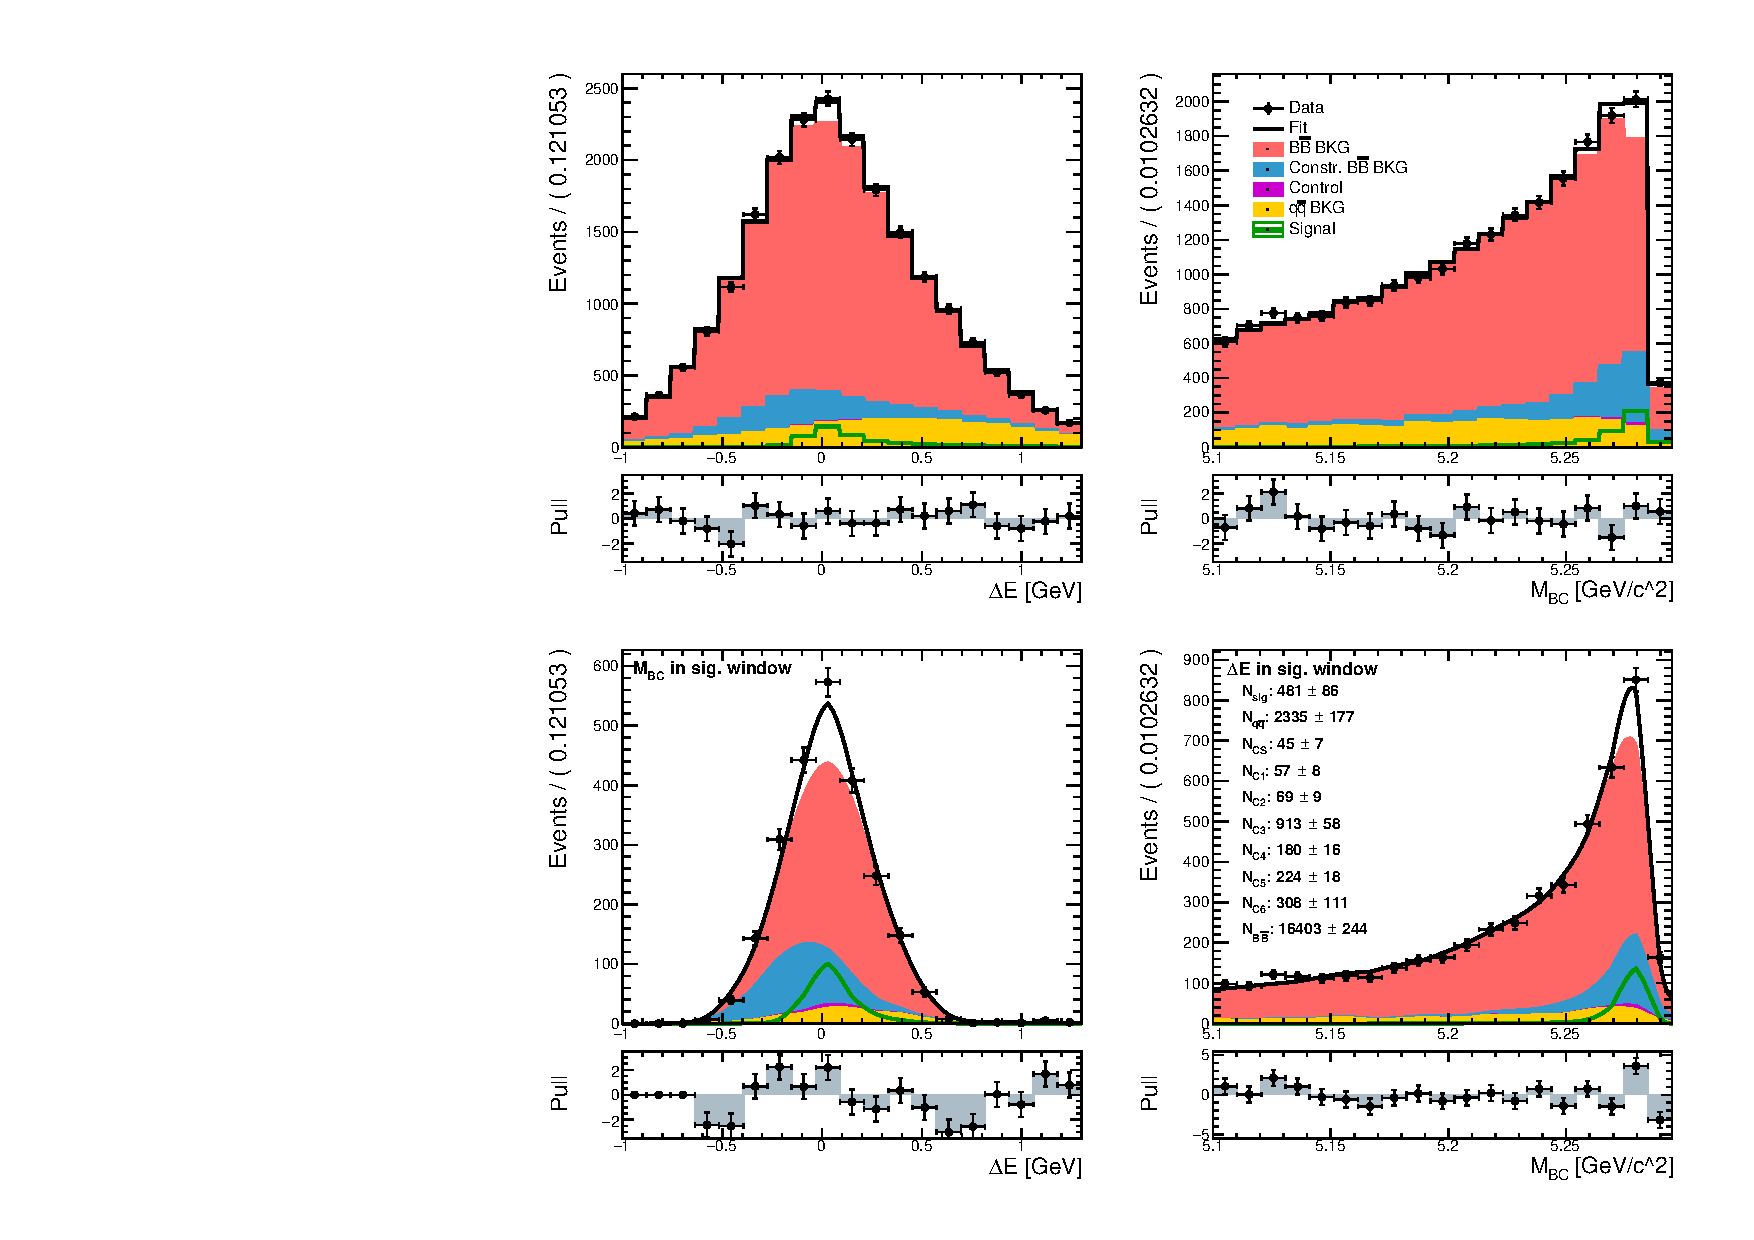
\includegraphics[width=\linewidth]{fig/sig_fit_data}
	\caption{Signal fit result on real data. Left column shows the $M_{BC}$ and the right column shows the $\Delta E$ distribution in the full fit window (top) and the signal window (bottom).}
	\label{fig:sig_fit_data}
\end{figure} 

\begin{table}[H]
	\centering
	\begin{tabular}{|l|l|}
		\hline
		Category & Fit Yield \\
		\hline
		Signal & $476 \pm 86$ \\
		\hline
		$q \bar q$ background & $ 2315 \pm 179 $ \\
		\hline
		$C_0$ & $ 45 \pm 7 $ \\
		\hline
		$C_1$ & $ 57 \pm 8 $\\
		\hline
		$C_2$ & $ 69 \pm 9 $ \\
		\hline
		$C_3$ & $ 910 \pm 57 $ \\
		\hline
		$C_4$ & $ 180 \pm 16 $ \\
		\hline
		$C_5$ & $ 223 \pm 18 $ \\
		\hline
		$C_6$ & $ 341 \pm 107 $ \\
		\hline
		Other $B \bar B$ background & $ 16399 \pm 246 $ \\
     	\hline
	\end{tabular}
	\caption{Yields of all signal fit contributions on data.}
	\label{tab:sig_yields}
\end{table}

\begin{table}[H]
	\centering
	\begin{tabular}{|l|l||l|l|}
		\hline
		Constraint & Value & Constrain & Value \\
		\hline
$\mathcal{B}_{0}$ & $0.049 \pm 0.001$ & $N_{30}$ & $103 \pm 10$\\
\hline
$\mathcal{B}_{1}$ & $1.076 \pm 0.004$ & $N_{31}$ & $211 \pm 14$\\
\hline
$\mathcal{B}_{2}$ & $0.021 \pm 0.001$ & $N_{32}$ & $136 \pm 12$\\
\hline
$\mathcal{B}_{3}$ & $1.014 \pm 0.018$ & $N_{33}$ & $267 \pm 16$\\
\hline
$\mathcal{B}_{4}$ & $1.018 \pm 0.010$ & $N_{34}$ & $19 \pm 4$\\
\hline
$\mathcal{B}_{5}$ & $1.439 \pm 0.063$ & $N_{35}$ & $35 \pm 6$\\
\hline
$\mathcal{B}_{6}$ & $1.092 \pm 0.038$ & $N_{40}$ & $48 \pm 7$\\
\hline
$\mathcal{B}_{7}$ & $1.035 \pm 0.008$ & $N_{41}$ & $7 \pm 3$\\
\hline
$\mathcal{B}_{8}$ & $0.971 \pm 0.038$ & $N_{42}$ & $99 \pm 10$\\
\hline
$\mathcal{B}_{9}$ & $1.052 \pm 0.038$ & $N_{43}$ & $10 \pm 3$\\
\hline
$\mathcal{B}_{10}$ & $0.945 \pm 0.029$ & $N_{44}$ & $14 \pm 4$\\
\hline
$\mathcal{B}_{11}$ & $1.331 \pm 0.441$ & $N_{45}$ & $3 \pm 2$\\
\hline
$N_{\mathrm{control}}^{MC}$ & $1179 \pm 11$ & $N_{50}$ & $103 \pm 10$\\
\hline
$N_{\mathrm{control}}$ & $1215 \pm 43$ & $N_{51}$ & $63 \pm 8$\\
\hline
$N_{00}$ & $44 \pm 7$ & $N_{52}$ & $31 \pm 6$\\
\hline
$N_{10}$ & $54 \pm 7$ & $N_{53}$ & $21 \pm 5$\\
\hline
$N_{11}$ & $6 \pm 2$ & $N_{60}$ & $69 \pm 8$\\
\hline
$N_{20}$ & $23 \pm 5$ & $N_{61}$ & $94 \pm 10$\\
\hline
$N_{21}$ & $41 \pm 6$ & $N_{62}$ & $63 \pm 8$\\
\hline
$N_{22}$ & $6 \pm 2$ & $N_{63}$ & $35 \pm 6$\\
\hline
	\end{tabular}
\caption{Mean values and standard deviations of constraints after the fit.}
\label{tab:constraints}
\end{table}

In this fit setup we perform a random smearing of the $\Delta E$ variable according to the Poisson distribution. The result is similar to a convolution with a Gaussian function, but the application is different in the sense that it returns a slightly different result after each fit. We perform 500 data fits in order to obtain the mean values of the signal yield and fit error. The averaged result is
\begin{equation*}
\bar N {}_{sig} = 487 \pm 86,
\end{equation*}
where the error represents the joint value of the statistical error as well as the systematic error of the Gaussian constraints used in the fit. 

%It is possible to estimate the size of the systematic errors from this contribution by fixing the Gaussian constraints to the mean values to obtain the pure statistical error. Due to the same reasons as above, we repeat the fit 500 times and subtract the mean statistical error from the initial error. The result with split errors is then
%\begin{equation*}
%\bar N {}_{sig} = 476 \pm 86.
%\end{equation*}

\subsection{Branching Ratio Calculation for Signal Decay}

Similarly as for the control decay, we are able to calculate the branching ratio of the signal decay via the formulas
\begin{align}
\mathcal{B}^{MC}_{\mathrm{sig}} &= \frac{N^{\mathrm{MC}}_\mathrm{sig} \times \epsilon_{MC}}{2N_{B\bar B}^{MC}},\\
\mathcal{B}_{\mathrm{sig}} &= \frac{N_\mathrm{sig} \times \epsilon_{MC} \times \rho_{PID}}{2N_{B\bar B}},
\label{eq:br_data_sig}
\end{align}
where $N^{\mathrm{MC}}_\mathrm{sig}$ and $N_\mathrm{sig}$ are yields of the signal fit on MC and data, $\epsilon_{MC}$ is the MC efficiency of the signal sample, $\rho_{PID}$ the PID correction factor, and $N_{B\bar B}^{MC}$ and $N_{B\bar B}$ are the numbers of $B \bar B$ meson pairs on MC and data, respectively.

The signal efficiency was determined on the same signal MC sample as was used throughout the analysis. The full signal efficiency is determined to be
\begin{equation*}
\epsilon_{MC} = ,
\end{equation*}

\begin{equation*}
\epsilon_{MC} = \frac{1}{N}\sqrt{n(1-\frac{n}{N})},
\end{equation*}






